\section{The plan}

\begin{figure}
	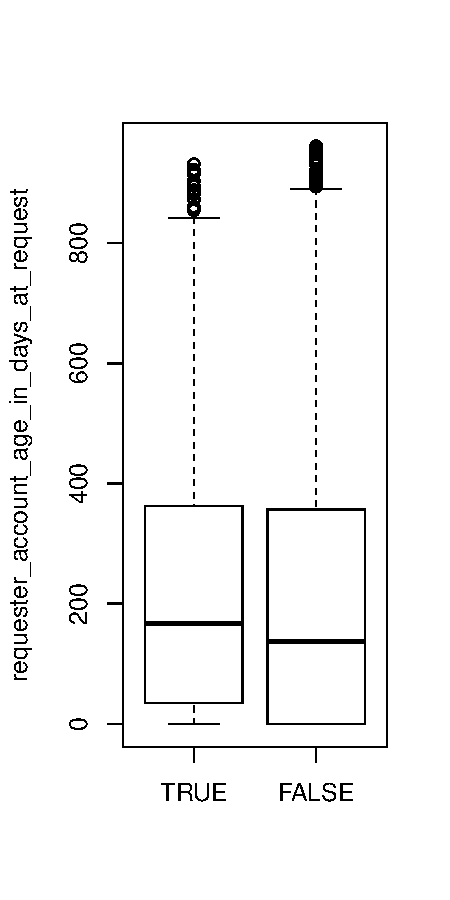
\includegraphics[width=0.19\textwidth]{data/requester_account_age_in_days_at_request}
	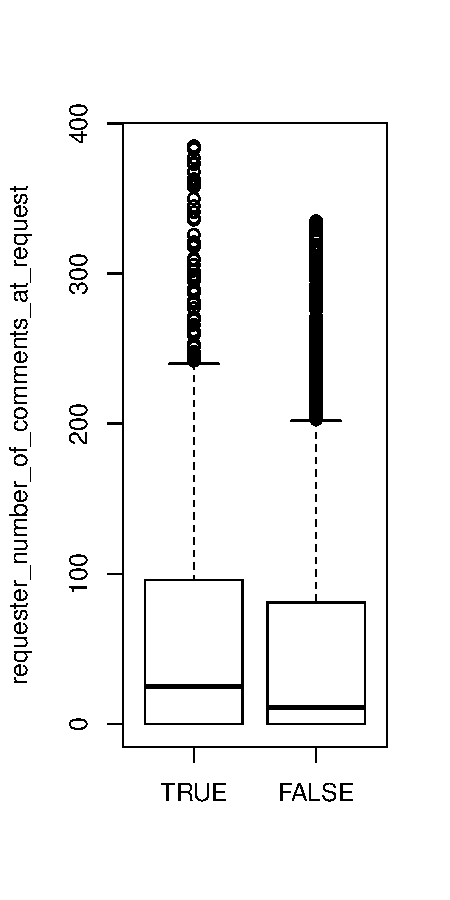
\includegraphics[width=0.19\textwidth]{data/requester_number_of_comments_at_request}
	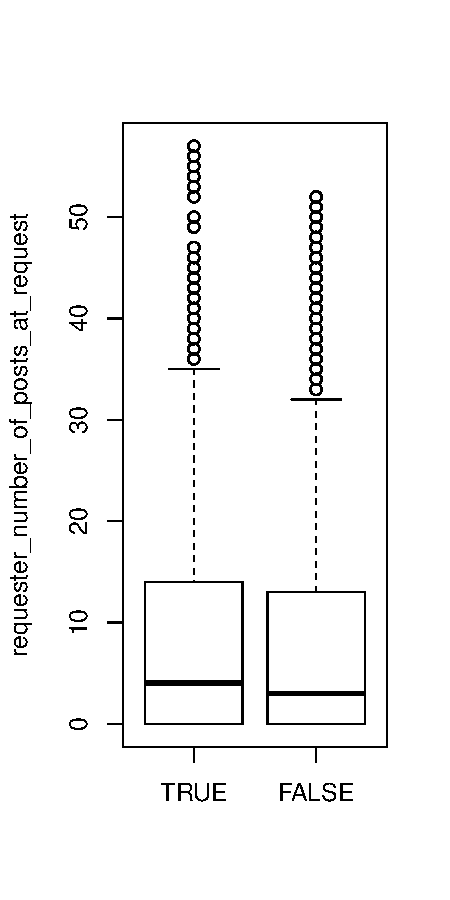
\includegraphics[width=0.19\textwidth]{data/requester_number_of_posts_at_request}
	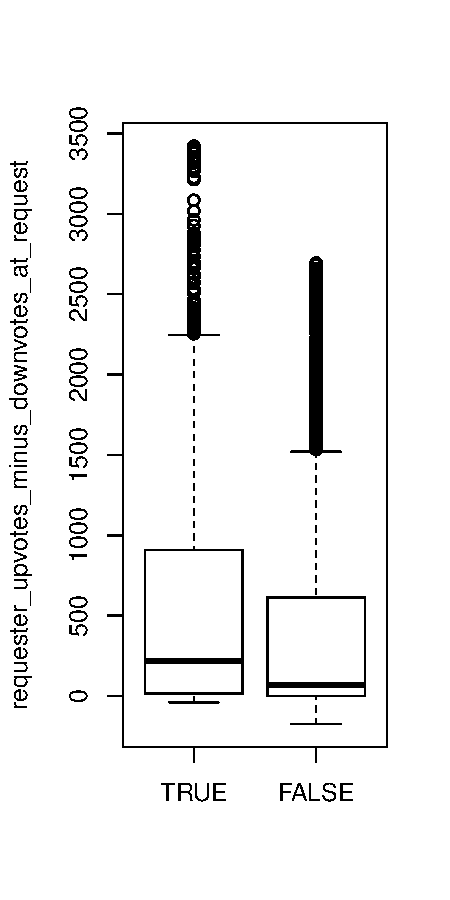
\includegraphics[width=0.19\textwidth]{data/requester_upvotes_minus_downvotes_at_request}
	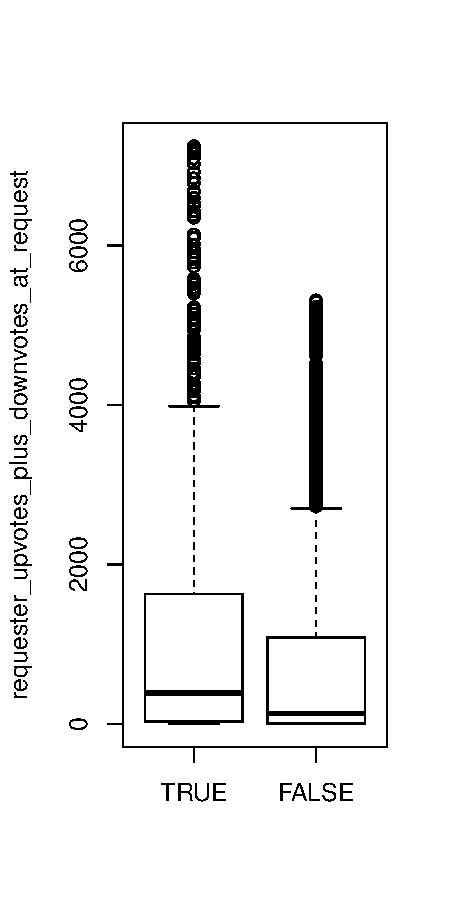
\includegraphics[width=0.19\textwidth]{data/requester_upvotes_plus_downvotes_at_request}
	\caption{Boxplots of some attributes based on the success of requests}
	\label{boxplot}
\end{figure}

To analyze our data we will perform three critical steps:

\begin{itemize}
	\item General analysis of simple information about requesters.
	\item General analysis of textual attributes (request subject and body).
	\item Apply prediction model to measure effectiveness of each factor.
\end{itemize}

For example, we could perform comparison between successful and unsuccessful requests to see if an older account holder will have more chance at receiving a free pizza or not using a simple box plot of the attribute \textit{requester\_account\_age\_in\_days\_at\_request}. Table~\ref{boxplot} is showing such analysis for the five most interesting attributes containing requester information. We will also apply prediction model such as logistic regression using different attribute to see which one have the best predictive power. Such analysis will give us some idea of how the information available in Reddit about the requesters could effect the outcome.\\

The two most interesting and valuable attributes in our dataset are \textit{request\_title} and \textit{request\_text\_edit\_aware}. These attributes contain the title and textual body of each request. Most of decision will be based upon the contents of these two attributes. We will first performing some preprocessing including:  tokenizing, stop-word removal, stemming... Then we will use a simple frequency based phrase builder to create phrases that occurred enough but not too much or too little (The details will be included in check point report). We could then investigate the relationship between terms and phrases that co-occur the most with successful and unsuccessful requests. We could also use simple logic regression to see which terms or phrases have the most predictive power.\\

Finally, we will apply Word2Vec on these textual attributes to extract vector representation of terms and phrases, then by using clustering we could be able to find cluster of terms and phrases that have similar syntactic and semantic meaning. We then extract the \q{bag-of-cluster} vector for each request and feed this to SVN so that the model can learn to predict the outcome. By investigate the weight vector of SVN model we will be able to tell which cluster (factor) have the most effect on the outcome.


